\documentclass[11pt,a4paper]{article}
\usepackage{amsmath,amssymb,graphicx,geometry,booktabs,hyperref}
\usepackage{setspace}
\onehalfspacing
\emergencystretch=1.5em
\geometry{margin=1in}

\title{\textbf{KIKO Through the Program:\\
What a Hedging Research Framework Says About Korea's\\
2008 Knock-In Knock-Out Disaster}}
\author{\textbf{Jihong Park} \\ Pusan National University}
\date{July 2026}

\begin{document}

\maketitle

\begin{abstract}
In 2008 the depreciation of the Korean won detonated a family of ``zero-cost'' currency structures (knock-in knock-out (KIKO) contracts, typically one purchased put against two written knock-in calls) on the balance sheets of hundreds of exporting firms, pushing many operationally profitable companies into distress. This note revisits the canonical 1-put-2-call KIKO with the machinery of a research program on corporate hedging: the budget-allocation framework's stress ledger and barrier survival haircut, the barrier-option engine's first-passage Monte Carlo and delta diagnostics, the IFRS~9 designation ledgers, and the disclosure-and-hedging equilibrium. Priced under the program's own FX calibration, a stylized KIKO at the geometry actually sold (strike two percent above the forward, knock-in seven percent above spot, double leverage) was not zero-cost: the two written calls were worth roughly twenty-seven times the knocked-out put they nominally financed, an inception transfer near five percent of notional. The protection leg dies in over ninety-five percent of the scenarios in which it is needed; the package carries a delta of $-0.8$ per dollar of notional on day one; and conditional on even a five-percent depreciation, the knock-in springs with probability $0.97$. Each of the program's four layers isolates one piece of the failure: budgeting on the premium ledger instead of the stress ledger, hedging Greeks that break at barriers, books that switch regime discontinuously at the knock-in, and disclosure rules that would have caught the notional-to-flow ratio only if they quantified exposure. The note's summary proposition: barriers convert market risk into survival risk, and in 2008 every layer of the firm priced survival risk incorrectly at the same time.
\end{abstract}

\noindent\textbf{Keywords:} KIKO; barrier options; knock-in; zero-cost collar; corporate hedging; suitability; hedge accounting; disclosure.\\
\textbf{JEL codes:} G32, G13, G28, M41.

\section{Introduction}
\label{sec:intro}

Between 2006 and 2008, as the won appreciated, Korean banks sold exporters a family of ``zero-premium'' currency structures marketed as enhanced forward hedges. The canonical form, the knock-in knock-out, or KIKO, packaged one purchased USD put (the protection the exporter wanted) with two written USD calls per put (the financing the exporter did not understand). Two barriers completed the design: the put was extinguished if the exchange rate ever fell through a lower barrier, and the written calls activated, at double notional, if the rate ever rose through an upper one. When the global financial crisis drove USD/KRW from the mid-900s to above 1{,}400 in late 2008, the knock-ins triggered en masse. Firms that had, in many documented cases, written structures on two to three times their actual dollar flows found themselves obligated to deliver dollars they did not have at strikes hundreds of won below market. Operationally profitable exporters failed; litigation ran for years.

This note asks a narrow question: \emph{what does a modern hedging research program, built for a different firm and a different risk, have to say about KIKO?} The program in question was built around a Korean crude-oil importer's joint WTI--currency exposure and has four components: a budget-constrained allocation framework with a stress ledger and a barrier survival haircut; a barrier-option pricing and delta-hedging engine built on first-passage Monte Carlo; an IFRS~9 cash-flow-hedge accounting engine that measures what designation choices do to the books when barrier events strike; and an equilibrium model of disclosure and hedging in which disclosure operates through the price of residual risk. None of these components models KIKO. The claim of this note is that each isolates, with numbers, one of the four layers on which KIKO's damage depended, and that the composite lesson is sharper than any single-layer account.

Section~\ref{sec:pricing} prices the structure honestly under the program's calibration and quantifies the inception transfer hidden inside ``zero cost.'' Section~\ref{sec:mortality} applies the survival-haircut logic to the protection leg. Section~\ref{sec:delta} examines the package's delta profile and what it implies about who could measure the position. Section~\ref{sec:books} traces the accounting, and Section~\ref{sec:disclosure} the disclosure regime that would -- and the ones that would not -- have surfaced the exposure. Section~\ref{sec:conclusion} states the composite proposition. Throughout, the exercise is deliberately stylized: a single-settlement one-year contract with continuous barrier monitoring, priced under the program's calibration rather than 2007 market data, with limitations collected in Section~\ref{sec:limits}.

\section{The Structure, Priced Honestly}
\label{sec:pricing}

\subsection{Setup}

The stylized KIKO is written on USD/KRW under the program's production calibration: spot $S_0=1{,}540.64$, volatility $\sigma=0.09258$, $r_{USD}=4.0\%$, $r_{KRW}=3.5\%$, horizon $T=1$ year, giving a forward $F=1{,}532.96$. The firm (an exporter with dollar flows) holds: long one put with strike $K$, extinguished if the spot ever trades at or below $L=0.95\,S_0=1{,}463.61$; short $n=2$ calls with strike $K$, activated if the spot ever trades at or above $U=1.07\,S_0=1{,}648.48$. Pricing is by the program's own method: risk-neutral GBM Monte Carlo, 200{,}000 paths at 260 steps per year, with a log-space Brownian-bridge first-passage correction on every barrier at every step, the same machinery the program's delta-hedging layer uses for its knock-out quanto, the FX leg carrying no jump component in the program's calibration.

\subsection{Three dials, one trap}

The structure has three free dials (the strike $K$, the knock-in $U$, and the leverage $n$), and the zero-cost condition $P_{put}^{KO}(K,L)=n\,C_{call}^{KI}(K,U)$ fixes one given the other two. Solving each way exposes the same trap from three angles:

\begin{table}[h]
\centering
\small
\begin{tabular}{llll}
\toprule
Fixed & Solved & Result & Reading \\
\midrule
$U=+7\%$, $n=2$ & $K^{*}$ & $F+9.8\%$ & an absurdly generous strike -- the visible bait \\
$K=F+2\%$, $n=2$ & $U^{*}$ & beyond $+25\%$ & an honest knock-in nobody would bother selling \\
$K=F+2\%$, $U=+7\%$ & $n^{*}$ & $0.075$ & the put deserves \emph{one-thirteenth} of one call \\
\bottomrule
\end{tabular}
\caption{Zero-cost parameterizations of the stylized KIKO under the program's calibration. The geometry actually sold in the episode (modest sweetener, tight knock-in, double leverage) is mutually inconsistent with zero cost: it corresponds to the third row with $n=2$ sold against a fair $n^{*}=0.075$.}
\label{tab:dials}
\end{table}

At the sold geometry ($K=1{,}563.62$, $U=1{,}648.48$, $n=2$), the legs price at $P_{put}^{KO}=3.01$ and $C_{call}^{KI}=39.89$ KRW per USD of notional. The knocked-out put is nearly worthless (the barrier destroys $95.8\%$ of the equivalent vanilla put's value ($71.45$)), while each written knock-in call, its barrier only seven percent away under a nine-percent volatility, is worth nearly a vanilla call. The ``zero-cost'' package therefore transferred
\begin{equation}
n\,C_{call}^{KI}-P_{put}^{KO} \;=\; 2(39.89)-3.01 \;=\; 76.8 \text{ KRW per USD} \;\approx\; 5.0\%\ \text{of notional}
\label{eq:margin}
\end{equation}
to the dealer at inception. On the program firm's monthly flow of \$157.88 million, that is roughly KRW 12 billion per tranche, paid invisibly, in option value rather than cash. The first finding is thus definitional: \emph{the sold KIKO was not a zero-cost hedge; it was a premium payment of about five percent of notional, disguised by the fact that no cash moved.} The budget-allocation paper's central discipline (that the constraint governs \emph{cost}, of which cash premium is only the visible ledger) is precisely the discipline whose absence this number measures.

\section{Protection That Dies When Needed}
\label{sec:mortality}

The program's allocation layer prices barrier cheapness with a survival haircut: a knock-out discount is worth taking only if the hedge's mortality \emph{in the states where it is needed} stays below the discount, and it measures, for its oil structure, a stress-conditional knock-out probability of $89.25\%$ against a break-even of $6.16\%$. The KIKO put leg fails the same test more spectacularly. Conditional on the terminal spot ending at or below $0.98\,S_0$ (the region where an exporter's protection begins to matter), the put has already been extinguished with probability $0.953$; at or below $0.96\,S_0$, probability $0.993$; conditional merely on the spot ending anywhere below its starting point, $0.898$ (Figure~\ref{fig:mortality}). The knock-out discount of $95.8\%$ is, by the survival-haircut logic, compensation for a protection leg whose delivery probability in its own coverage zone is a few percent. The put was not cheap insurance; it was an expensive lottery ticket printed on insurance paper.

\begin{figure}[h]
\centering
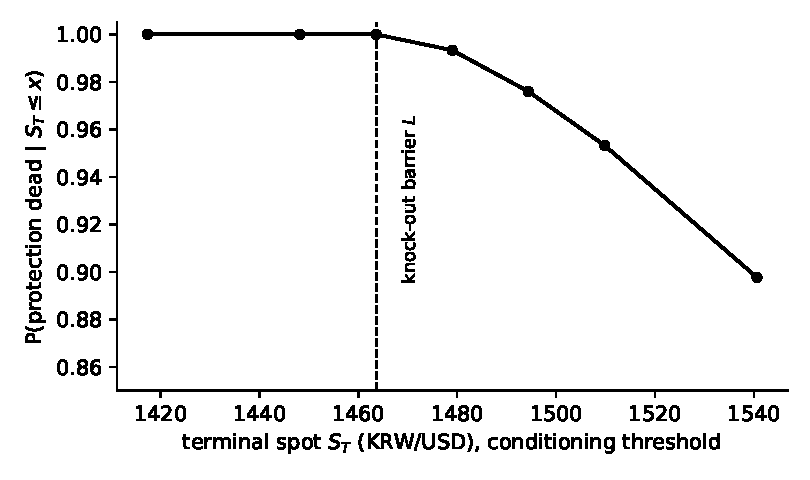
\includegraphics[width=0.62\textwidth]{figures/fig_kiko_mortality.pdf}
\caption{Protection mortality: probability the knocked-out put is already dead, conditional on the terminal spot ending at or below $x$. The knock-out barrier sits at $L=1{,}463.6$.}
\label{fig:mortality}
\end{figure}

\section{A Position Wearing a Hedge's Name Tag}
\label{sec:delta}

The delta-hedging layer's subject is the fragility of barrier-option Greeks: different estimators of the same delta diverge by double digits near inception, and the divergence is a structural property of discontinuous payoffs, not an implementation defect. The KIKO package makes the point without any estimator subtlety at all. Figure~\ref{fig:delta} plots the package's delta per dollar of notional across spot levels. At inception the ``hedge'' already carries $\Delta=-0.82$: the two knock-in calls, live with probability $0.43$ over the year, dominate the nearly-dead put from the first day. An exporter holding one dollar of operating flow ($+1$) plus the package holds a \emph{net} delta of $+0.18$; and by a twelve-percent depreciation the package is at $-1.66$, the net position at $-0.66$: \textbf{the instrument sold as depreciation protection makes its holder short depreciation}. Conditional on even a five-percent depreciation over the year, the knock-in has sprung with probability $0.968$; at ten percent, $1.000$. There is no path to the loss states that does not pass through the trigger.

\begin{figure}[h]
\centering
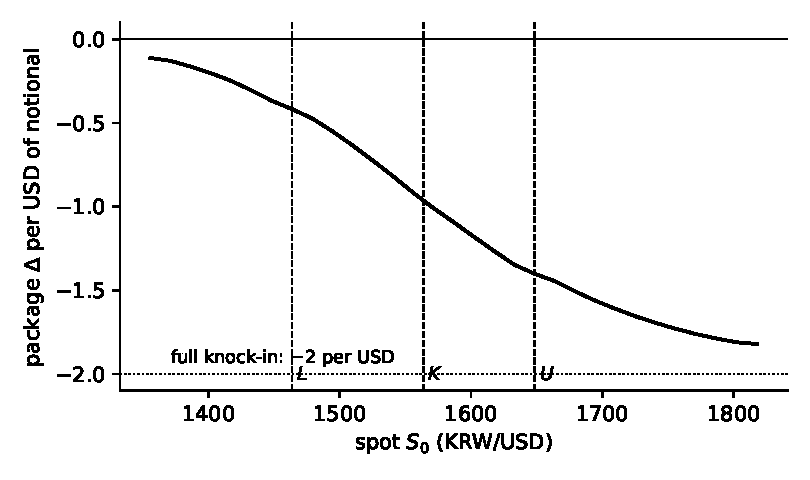
\includegraphics[width=0.62\textwidth]{figures/fig_kiko_delta.pdf}
\caption{Package delta per USD of notional across spot levels at inception (sold geometry). Dashed verticals mark $L$, $K$, $U$; the dotted line is the fully knocked-in limit of $-2$.}
\label{fig:delta}
\end{figure}

The stress ledger completes the account (Figure~\ref{fig:ladder}). At a $+25\%$ depreciation an unlevered exporter hedged one-for-one loses a net 339 KRW per dollar of flow: the operating windfall of 385 swamped by a package loss of 724. At the overhedge ratios documented in the episode (2--3$\times$ flow), the same move costs 1{,}426 KRW per dollar of \emph{actual} flow, and a $+50\%$ move costs 2{,}966, roughly two years of a healthy exporter's operating margin, incurred in months. This is the arithmetic of profitable firms failing.

\begin{figure}[h]
\centering
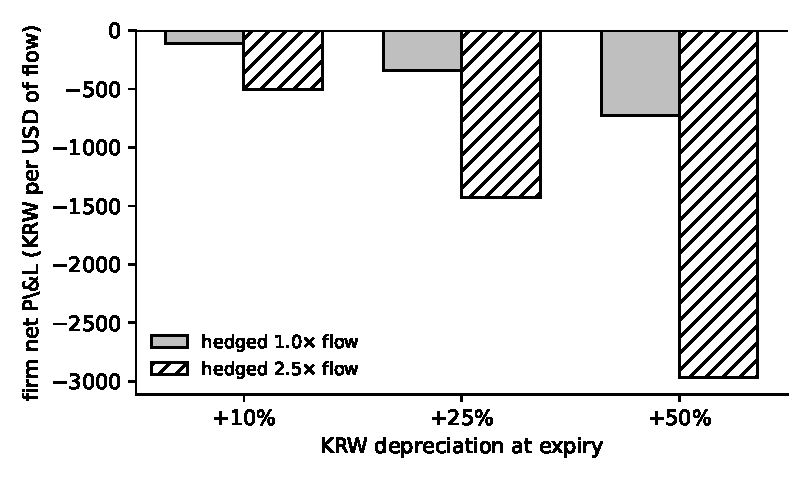
\includegraphics[width=0.62\textwidth]{figures/fig_kiko_ladder.pdf}
\caption{Firm net P\&L per USD of operating flow at expiry, by depreciation scenario and hedge multiple (package at sold geometry; knock-in triggered on the path to each scenario).}
\label{fig:ladder}
\end{figure}

The measurement asymmetry is the deeper point. The dealer side of this trade ran barrier engines of exactly the kind the program's delta-hedging layer builds, and that layer documents how hard the Greeks are to pin down \emph{even then}. The corporate side typically ran nothing: no mark-to-market, no scenario ladder, no barrier-hit probabilities. A workable suitability principle falls out of the program's language: \emph{if the uncertainty band on your own estimate of the position's delta, times its notional, exceeds your equity buffer, the position does not belong on your balance sheet} -- and a firm that cannot form the estimate at all fails the test by construction.

\section{The Books: A Regime Switch at the Barrier}
\label{sec:books}

The IFRS~9 paper's engine exists to measure what designation choices do when barrier events strike a hedging book: its headline exhibits include the discontinuous migration of an instrument out of hedge treatment on a knock-out, and the earnings volatility injected when a surviving leg is carried at fair value through profit or loss thereafter. KIKO is that mechanism at maximum amplitude, with three aggravations. First, the written double-call leg could never have qualified for hedge accounting: a 2$\times$ short against a 1$\times$ exposure fails effectiveness arithmetic by construction, so the loss engine sat at FVTPL from day one, yet the package was internally narrated, and often booked, as ``the hedge.'' Second, the knock-in is a regime switch of the books as well as of the economics: a contingent liability that had lived in disclosure footnotes became a realized, growing derivative liability on the face of the statements in a single quarter. Third, and most practically, the gap the accounting could not show is exactly what the paper's economic-residual layer ($\sigma_{econ}$) is designed to measure: the distance between the hedged story the ledgers told and the levered short the firm actually held. The episode's ``sudden'' losses were sudden only on paper; the exposure had been continuously present and continuously unmeasured.

\section{The Disclosure That Would Have Caught It}
\label{sec:disclosure}

The disclosure layer's equilibrium delivers one sharp policy result: mandates move hedging behavior only through the margin that quantifies the priced exposure: floors on orthogonal content produce an exact zero, a prediction verified on two realized Korean mandates. Run backwards over KIKO, the result sorts post-crisis regulatory instincts into two bins. Checkbox disclosure (``does the firm use derivatives?'', governance attestations, qualitative risk statements) sits on the orthogonal margin; the model predicts, and its executed nulls illustrate, that it changes nothing. The quantity that would have surfaced KIKO before it detonated is a single ratio: \emph{derivative notional to underlying flow}, per currency, marked against its barriers. Firms carrying $2.5\times$ overhedges with knock-ins seven percent away were, in the model's language, carrying an enormous unpriced $R$ that quantified disclosure would have moved directly into $\Lambda$ (the price their banks, boards, and auditors attached to residual risk) years before the barrier was touched. The KIKO episode is thus the disclosure layer's exposure-quantification ladder read as history: the rungs that existed in 2007 were orthogonal, and the rung that mattered did not exist.

\section{Conclusion: One Proposition, Four Layers}
\label{sec:conclusion}

\begin{quote}
\emph{Barriers convert market risk into survival risk, and in 2008 every layer of the firm priced survival risk incorrectly at the same time.} Budgeting priced the premium ledger and missed a five-percent-of-notional transfer (Section~\ref{sec:pricing}) and a protection leg with near-certain mortality in its own coverage zone (Section~\ref{sec:mortality}). Trading assumed smooth exposures and held a package that was short its own hedging objective from inception (Section~\ref{sec:delta}). Accounting told a hedged story until the knock-in forced a discontinuous regime switch (Section~\ref{sec:books}). And disclosure rules asked every question except the one ratio that mattered (Section~\ref{sec:disclosure}).
\end{quote}

Each layer's failure was individually survivable; their coincidence was not -- and their coincidence was not an accident, because all four mispricings share a single root: the state-contingency that barriers introduce is invisible to tools built for linear instruments. That is also why the remedy is architectural rather than product-level. A firm whose budget process carries a stress ledger, whose instrument desk publishes barrier-hit odds, whose books measure the residual between economics and designation, and whose disclosures quantify notional against flow (a firm, that is, whose four layers share one state) cannot buy a KIKO by accident. It can still buy one on purpose; no framework prevents a deliberate levered bet. What the program's machinery removes is the 2008 configuration: the deliberate bet that eight hundred treasurers believed was a hedge.

\section{Limitations}
\label{sec:limits}

The reconstruction is stylized in five respects. The contract is single-settlement at one year with continuously monitored barriers, where the sold products were typically monthly-settling strips over one to three years with per-window observation; the strip structure compounds rather than mitigates the mechanisms shown. Pricing uses the program's calibration ($\sigma=9.26\%$, 2020s rates) rather than 2007 market data; pre-crisis implied volatilities were lower, which shrinks every level in Sections~\ref{sec:pricing}--\ref{sec:delta} but changes no sign and no ordering, and the episode itself was precisely a realization far outside the implied distribution that priced the products. The exporter's operating exposure is treated as a fixed dollar flow, ignoring the volume channel through which depreciation raises export revenue. Credit, collateral, and margin-call dynamics, a major amplifier in the episode, are absent. And the note takes no position on the legal questions the episode generated; its subject is measurement, not intent.

\begin{thebibliography}{9}

\bibitem{broadie1996} Broadie, M., and P. Glasserman (1996). ``Estimating Security Price Derivatives Using Simulation.'' \emph{Management Science} 42(2), 269--285.

\bibitem{garman1983} Garman, M. B., and S. W. Kohlhagen (1983). ``Foreign Currency Option Values.'' \emph{Journal of International Money and Finance} 2(3), 231--237.

\bibitem{merton1976} Merton, R. C. (1976). ``Option Pricing When Underlying Stock Returns Are Discontinuous.'' \emph{Journal of Financial Economics} 3(1--2), 125--144.

\bibitem{stulz1996} Stulz, R. M. (1996). ``Rethinking Risk Management.'' \emph{Journal of Applied Corporate Finance} 9(3), 8--25.

\end{thebibliography}

\end{document}
